\documentclass[__main__.tex]{subfiles}

\begin{document}

\qtitle{Ч}{07}
Факторизованные и запутанные состояния. Проекторная техника. Неравенства Белла.\\ 

\textbf{Факторизованные и запутанные состояния}

Рассмотрим спиновое пространство состояний системы из двух электронов. Так как электроны являются фермионами с s = $\frac{1}{2}$, то число возможных проекций на выделенное направление равно $2s + 1 = 2$. Получаем, что размерность спинового пространства каждого электрона равна 2, т. е все пространство можно описать с помощью двух базисных векторов $|+\rangle_1$, $|-\rangle_1$\\

$|st\rangle_1 = {}^1 C_{+} |+\rangle_1 + {}^1 C_{-} |-\rangle_1$ - состояние 1-го электрона. ${}^1 C_{+}$ и ${}^1 C_{-}$ являются комплексными константами. Единицы указывают на то, что речь идет о 1-м электроне. \\

Аналогично $|stt\rangle_2 = {}^2 C_{+} |+\rangle_2 + {}^2 C_{-} |-\rangle_2$ - cостояние 2-го электрона. Дополнительная буква t подчеркивает (это идея Никифорова, не моя), что $|st\rangle_1$ и $|stt\rangle_2$ не совпадают.\\

Состояние каждого отдельного электрона можно описать с помощью двух параметров (4 - 1 - 1 = 2 (4 параметра исходно из-за того, что параметры комплексные, 2 параметра отбрасываются из-за нормировки и выбора фазы). \\

Общее состояние составной системы $|Gst\rangle$ в некоторых случаях можно представить в форме \textbf{факторизованного состояния} $|fst\rangle = |st\rangle_1 |stt\rangle_2$ (в виде тензорного произведения (знак опущен) состояний каждого элемента системы) и может быть описано с помощью 4 параметров:\\

$$|Gst\rangle = {}^1C_{+}{}^2C_{+}|++\rangle + {}^1C_{+}{}^2C_{-}|+-\rangle + {}^1C_{-}{}^2C_{+}|-+\rangle + {}^1C_{-}{}^2C_{-}|--\rangle$$.

Общее состояние системы $|Gst\rangle$ описывается как суперпозиция базисных векторов $\lbrace |++\rangle, |+-\rangle, |-+\rangle, |--\rangle \rbrace$:

$$|Gst\rangle = C_{++}|++\rangle + C_{+-}|+-\rangle + C_{-+}|-+\rangle + C_{--}|--\rangle$$.

и описывается $2 \cdot 4 - 1 - 1 = 6$ параметрами (вычитаем единицу два раза из-за нормировки, 2 - так как константы комплексные, 4 - так как констант всего 4) . Получаем, что не все состояния системы можно представить в виде произведения состояний системы. Это приводит к наличию \textbf{запутанных cостояний}.\\

\textit{Пример факторизованного состояния}

$$|Fst\rangle = \alpha |+-\rangle$$

Нормировка: $1 = \langle Fst | Fst \rangle  = | \alpha |^2 {}_1 \langle + + | + + \rangle_1 {}_2 \langle - - | - - \rangle_2 \Rightarrow \alpha = e^{i\beta}$

Можно выбрать любую фазу, например $\beta = 0$: $|Fst\rangle = |+-\rangle$

\textit{Пример запутанного состояния}

$$|Est\rangle = \alpha \left(|+-\rangle - |-+\rangle\right) \; \Rightarrow \; \langle Est | = \left(\langle + - | - \langle - + |\right) \alpha^{*}$$

Условие нормировки: $1 = \langle Est | Est \rangle  = | \alpha |^2 \left( \langle + - | + - \rangle - \langle + - | - + \rangle - \langle - + | + - \rangle + \langle - + | - + \rangle \right) \; \Rightarrow \; \alpha = \frac{e^{i\beta}}{\sqrt{2}}$.

Так как можно выбрать любую фазу (напр. $\beta = 0$), то: $|Est\rangle = \frac{|+-\rangle - |-+\rangle}{\sqrt{2}}$

Вероятность в результате измерения обнаружить систему в состоянии $|+-\rangle$ составляет $\frac{1}{2}$, с той же вероятностью можно обнаружить систему в состоянии $|-+\rangle$. При этом, в то время как состояния единой системы полностью определено, ни одна из подсистем не находится в определенном состоянии.\\

Допустим, обнаруживается, что 1-й электрон находится в состоянии $|+\rangle_1$, тогда понятно, что 2-й находится в состоянии $|-\rangle_2$. Когда проводится измерение, запутанное состояние:

$$|Est\rangle = \frac{|+-\rangle - |-+\rangle}{\sqrt{2}}$$

коллапсирует в состояние $|Pst\rangle = |+-\rangle$. То есть при измерении, проводимом над 1-м электроном, определяется состояние 2-го электрона, причем \textit{мгновенно}, это называется \textbf{квантовой нелокальностью}.

\textbf{Проекторная техника}

\begin{definition}
Оператор $\hat{P}$ называется проектором, если он эрмитов ($\hat{P}^+ = \hat{P}$) и идемпотентен ($\hat{P}^2 = \hat{P}$).
\end{definition}

\begin{definition}
Оператор $\hat{P}_w$ называется проектором на подпространство $W$, если $\hat{P}_w |v\rangle = |w\rangle$.
\end{definition}

Пусть $|u\rangle = |w\rangle + |\varepsilon\rangle$, где $|u\rangle \in V$, $|w\rangle \in W$, $|\varepsilon\rangle \in \Sigma$, тогда:

$$\langle u | \hat{P}_w | v \rangle = \langle u | w \rangle = \langle w | w \rangle$$,
$$\langle v | \hat{P}_w | u \rangle^{*} = \langle v | w \rangle^{*} = \langle w | w \rangle$$

Так как $\langle u | \hat{P}_w | v \rangle = \langle v | \hat{P}_w | u \rangle^{*}$, то $\hat{P}^{+}_w = \hat{P}_w$

$$\hat{P}^2_w | v \rangle = \hat{P}_w \left(\hat{P}_w | v \rangle \right) = \hat{P}_w | w \rangle = |w\rangle = \hat{P}_w | v \rangle \; \Rightarrow \; \hat{P}^2_w = \hat{P}_w$$

Следовательно, оператор $\hat{P}_w$ является эрмитовым и идемпотентным, а значит удовлетворяет первому определению. 

\textbf{Неравенство Белла}

Если следовать логике ЭПР (парадокс , то еще до измерения спина у электрона есть определенное значение проекции спина.

Р/м три ``свойства'' электрона: проекция его спина вдоль $z$ (A), проекция его спина вдоль $x$ (B) и проекция спина электрона вдоль направления которое лежит в плоскости $OXZ$ и проходит под углом 45 градусов к осям $x$ и $z$ (C). Если перечисленные характеристики верны до эксперимента, то множество всех электронов можно разбить на классы 1-7 (cм. рисунок).\\

\begin{wrapfigure}[14]{R}{0.4\linewidth}
	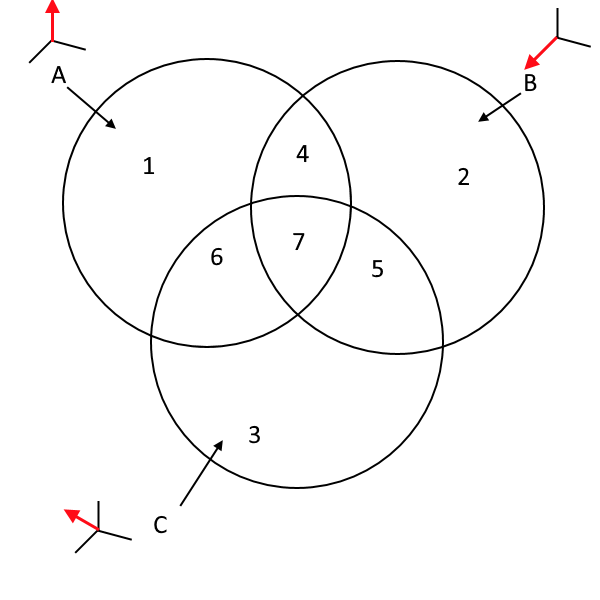
\includegraphics[width=1\linewidth]{img/Ч-07_1}{}
\end{wrapfigure}

Введем обозначение $N(A \cap \bar{C})$ - число элементов, обладающих свойством A и не обладающих свойством C.

Из этого следует, что справедливо следующее неравенство: $N(A \cap \bar{C}) + N(C \cap \bar{B}) \ge N(A \cap \bar{B})$

Рассмотрим систему из двух электронов, которая находится в состоянии $|Est\rangle = \frac{|+-\rangle-|-+\rangle}{\sqrt{2}}$, тогда если при измерении проекции спина 2-го электрона на направление $n_2 = \frac{1}{\sqrt{2}}(1, 0, 1)$ получится результат (С) (вдоль $n_2$), то проекция спина у 1-го будет против $n_2$ ($\neg C$). Таким образом, можно получить недостающую информацию о проекции спина электрона. Тогда неравенство, записанное выше можно переписать в форме:

$$N(A; C) + N(C; B) \ge N(A, B)$$,

Это неравенство является одним из неравенств Белла.

Квантовая механика предсказывает, что:

$N(A; С)$ пропорционально $\langle {}^1 \hat{P}_A \otimes {}^2\hat{P}_C \rangle = \frac{\langle+-|-\langle-+|}{\sqrt{2}} \cdot \frac{{}^1\hat{\sigma_z} + {}^1 \hat{1}}{2} \otimes \frac{\frac{{}^2 \hat{\sigma}_x + {}^2 \hat{\sigma}_z}{\sqrt{2}} + {}^2 \hat{1}}{2} \cdot \frac{|+-\rangle - |-+\rangle}{\sqrt{2}} =$\\
$=\frac{2 - \sqrt{2}}{8}$

$N(C; B)$ пропорционально $\langle {}^1 \hat{P}_C \otimes {}^2\hat{P}_B \rangle = \frac{\langle+-|-\langle-+|}{\sqrt{2}} \cdot \frac{\frac{{}^1 \hat{\sigma}_x + {}^1 \hat{\sigma}_z}{\sqrt{2}} + {}^1 \hat{1}}{2} \otimes  \frac{{}^2\hat{\sigma_x} + {}^2 \hat{1}}{2} \cdot \frac{|+-\rangle - |-+\rangle}{\sqrt{2}} =$\\
$=\frac{2 - \sqrt{2}}{8}$

$N(A; B)$ пропорционально $\langle {}^1 \hat{P}_A \otimes {}^2\hat{P}_B \rangle =  \frac{\langle+-|-\langle-+|}{\sqrt{2}} \cdot  \frac{{}^1\hat{\sigma_z} + {}^1 \hat{1}}{2} \otimes  \frac{{}^2\hat{\sigma_x} + {}^2 \hat{1}}{2} \cdot  \frac{|+-\rangle - |-+\rangle}{\sqrt{2}} =$\\
$ = \frac{1}{4}$

Получаем, что $N(A, C) + N(C, B) < N(A, B)$, т.е неравенство не выполняется.

Противоречие между ЭПР и квантовой механикой был разрешен в пользу последней экспериментальным путем.

\end{document}
